\section{Datenvorverarbeitung}
\label{dv}
Wie in den Grundlagen der Datenvorverarbeitung (vgl. \vref{aufbereitung}) beschrieben, ist diese Phase von besonderer Bedeutung für die Güte der \gls{dm}-Resultate. Es gilt, die Qualität der zuvor selektierten Zieldaten durch den Einsatz von geeigneten Verfahren nachhaltig zu verbessern und diese in einem für die \gls{dm}-Methode passendem Format bereitzustellen. Dazu müssen im Folgenden die Daten (in Form der selektierten Schüsse) zunächst von Fehlern bereinigt (siehe Data Cleaning \vref{datac}), anschließend fehlerfrei mit den Daten aller anderen verfügbaren Spielen zusammengeführt (siehe Data Integration \vref{datai}) und schließlich auf eine verwertbare Datenmenge reduziert werden (siehe Data Reduction \vref{datar}).

\subsection{Data Cleaning}
\label{datac}
Das Data Cleaning beschäftigt sich mit der durch fehlende, verrauschte und inkonsistente Daten (vgl. \vref{dc}) auftuenden Problematik. Diese werden nachfolgend näher untersucht und behandelt. 

\paragraph{Fehlende Daten}
Das ein ganzes Event, wie in diesem Falle ein Schuss, überhaupt nicht erfasst wird, ist sehr unwahrscheinlich, da Opta als marktführender Datenprovider großen Wert auf Akkuratesse und Vollständigkeit der bereitgestellten Daten legt. Für eine exakte Überprüfung müssten über 90.000 Spielminuten (\textit{34 Spieltage $\cdot$ 3,5 Saisons $\cdot$ 9 Spiele pro Spieltag $\cdot$ 90 Minuten}) händisch darauf geprüft werden, was sich aus zeitlichen Ressourcen nicht realisieren lässt	. Fehlen \glqq lediglich\grqq~einzelne Attribute in einem Datensatz, wie beispielsweise die x-Koordinate des Schusses, können diese Datensätze auf unterschiedliche Weise bearbeitet werden (siehe \vref{dc}). Ebenso könnte in diesem Fall das fehlende Attribut wieder manuell eingefügt werden, wodurch allerdings wieder ein zeitintensiver Vorgang entsteht. Die Verwendung von globalen Konstanten, Durchschnitts- oder Erwartungswerten als Ersatz für das fehlende Attribut würde aufgrund der Einzigartigkeit eines Schusses wiederum in einer Verzerrung der Realität enden. Infolgedessen wird solch ein Datensatz gänzlich ignoriert, da dieser vielmehr zu einer Verfälschung als zu einer Verbesserung des Modells führt. Die Datensätze aller 15.000 verfügbaren Schüsse sind vollständig und nicht von fehlenden Daten bzw. Attributen betroffen. Sollte beispielsweise ein Qualifier für die Identifizierung eines Elfmeters fehlen, muss geprüft werden, ob die Positionsdaten des Schusses gleich denen des Elfmeterpunktes sind und unmittelbar ein Foulspiel vorangegangen ist, um diesen Schussversuch anschließend manuell abgleichen zu können.\footnote{Dieser Fall trat insgesamt lediglich einmal ein.} Solche Adaptionen führen allerdings zu einem zeitaufwendigen Vorgang, da vorangegangen Events zur Validierung miteinbezogen werden. Letztlich muss auf die Qualität der Daten vertraut und mögliche Fehlervarianzen akzeptiert werden.

\paragraph{Verrauschte Daten und Ausreißer}
Ausreißer bezeichnen Daten, die erheblich von den vorliegenden Daten abweichen. Ob solche Ausreißer folglich ausgeblendet, adaptiert oder im Originalzustand verwendet werden sollten, hängt dabei vom konkreten Data-Mining-Kontext ab. \vref{outlier_shots} (Eigentore sind ausgeschlossen) zeigt dazu rot-umkreist die Ausreißer unter den Torerfolgen. Diese 	 heben sich deutlich von der Grundgesamtheit der gruppierten Torerfolge in der Nähe des gegnerischen Tores ab. Beispielsweise traf Moritz Stoppelkamp vom SC Paderborn in der Partie gegen Hannover 96 im Herbst 2014 mit seinem Schuss aus einer Distanz von 84 Metern, welcher bis heute einen Rekord in der deutschen Bundesligageschichte einnimmt.\seFootcite{Vgl.}{}{DeutscherFuballBund.2014} Dieser seltene aber entscheidende Torerfolg demonstriert die Relevanz der Behandlung solcher Daten. Aus einer Entfernung von 84 Metern wird selten bis überhaupt nicht auf das gegnerische Tor geschossen. Sollte jedoch, wie in diesem Fall, solch ein Versuch in einem Torerfolg resultieren, so grenzt die relative Häufigkeit\footnote{Absolute Häufigkeit (Torerfolge) geteilt durch die Anzahl aller Objekte der Menge (alle Schussversuche).} in diesem Bereich an die 100\%, was wiederum für eine hohe Wahrscheinlichkeit für einen Torerfolg sprechen würde. Dies ist dadurch begründet, dass es nahezu keine Schussversuche und damit auch keine Fehlversuche aus dieser Distanz gibt. Zur Erkennung solcher Ausreißer stehen, wie in \vref{dc} aufzeigt, einige Verfahren zur Verfügung, welche sich auf eindimensionale Datensätze einfach anwenden lassen. Durch die Zweidimensionalität des Koordinatensystems und der Tatsache, dass sich die Schussversuche beispielsweise nicht durch eine multiple Regressionsfunktion ausdrücken lassen (siehe \vref{outlier_shots}), müssen die Ausreißer manuell identifiziert werden (\textit{visuelles \gls{clustering}}), wobei das Ausmaß der deutlich abweichenden Torerfolge noch handhabbar ist. Die Entwicklung eines Algorithmus für die Erkennung solcher Ausreißer in der vorliegenden Datenmenge würde den Rahmen dieser Arbeit übersteigen. Die Anpassung der Ausreißer an die umliegenden Daten führt nur dann zum Erfolg, wenn genügend Schussversuche aus diesem Bereich vorliegen. Ferner würde die Verwendung des Originalzustands des Schusses zu einer Verfälschung führen, sodass diese Schüsse bei der Modellierung manuell ausgeschlossen werden müssen. Dazu stellt \gls{matlab} innerhalb des \gls{cft} ein entsprechendes Werkzeug für die Entfernung von Ausreißern bereit.

\begin{sidewaysfigure}[H]
\centering
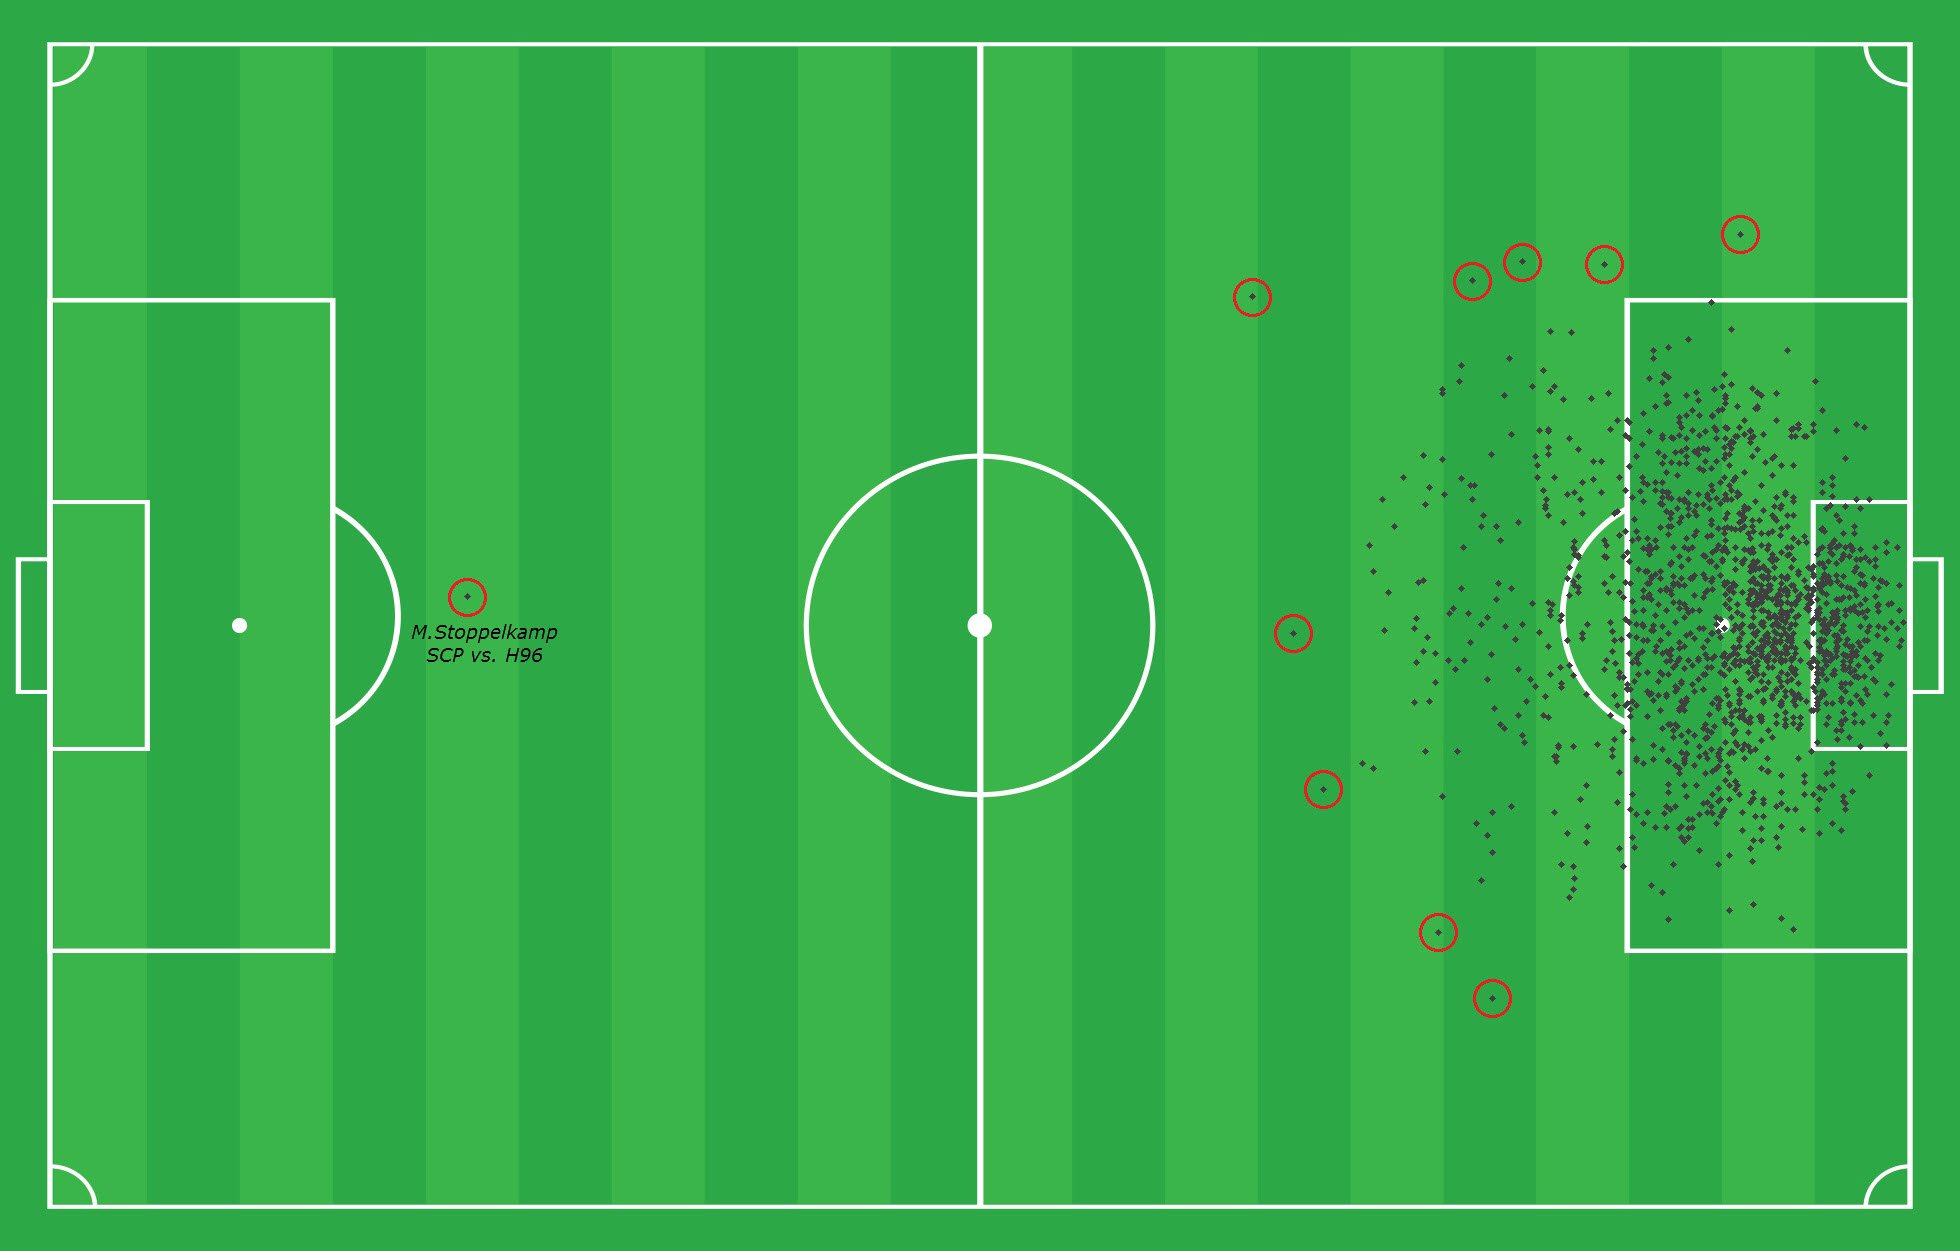
\includegraphics[scale=0.4]{se-wa-jpg/outlier_shots}
\caption[Darstellung der Ausreißer bei Torerfolgen]{Darstellung der Ausreißer bei Torerfolgen}
\label{outlier_shots}
\end{sidewaysfigure}

\paragraph{Inkonsistente Daten} 
Datensätze bei denen Attribute außerhalb des Wertebereichs liegen, wie beispielsweise negative Koordinaten oder bei denen der Wert größer als 100 ist, können durch Löschen entfernt oder durch die Zuhilfenahme anderer Datensätze sinnvoll ersetzt werden. Dazu werden alle Schüsse auf konsistente Koordinaten geprüft und im Fehlerfall manuell behandelt, wobei lediglich bei zwei Schüssen dieser Fall eingetreten ist. Wurden die Koordinaten falsch erfasst, ein Qualifier inkorrekter Weise gesetzt bzw. nicht gesetzt, müssten alle Schüsse erneut geprüft werden, was wie erwähnt einen nicht realisierbaren Vorgang darstellt. In solchen Fällen kann die Konsistenz der Daten nicht festgestellt bzw. aufgedeckt werden, sodass vermeidliche Fehler toleriert werden müssen.

\paragraph{Problem der weißen Linien} 
Im Rahmen dieser Arbeit wurde abseits der Aufgabestellung eine Problematik bei der Erkennung von Events, die direkt auf einer Linie stattfanden, eruiert. Anlass dazu gab die Visualisierung aller Torschüsse, wodurch ein Muster entlang der Spiellinien festgestellt wurde. Die im Anhang (siehe \vref{lines}) Darstellung aller Pässe - über 700.000 - bestätigt die Annahme, dass entlang der Linien des Spielfeldes die Events ungenau erfasst werden. Dies ist dadurch zu begründen, dass die automatische Videoverarbeitung den weißen Ball auf der weißen Linie nur schlecht bis gar nicht erkennen kann. Infolgedessen müssen auch bei den Schüssen kleine, jedoch vorhandene Koordinatenabweichungen hingenommen werden.
	
\subsection{Data Integration}
\label{datai}
In dieser Phase werden die selektierten und aufbereiteten Daten der einzelnen Spiele zu einer einzigen Datenquelle zusammengeführt. Bei der Konkatenation der Spiele muss auf ein einheitliches Format der Datensätze geachtet werden. Da alle von Opta bereitgestellten Spieldaten die gleiche Formatierung besitzen (hierzu zählen gleichnamige Attributsnamen und -werte), treten keine Identifikationsprobleme von Entitäten oder Konflikte bei Attributswerten auf. Jedes Event ist genau einem Spiel zugeordnet und kann über eine eindeutige ID identifiziert werden, sodass Duplikate ausgeschlossen werden können.
\newpage

\subsection{Data Reduction}
\label{datar}
Um die Effizienz der Regressionsanalyse zu steigern und zugleich die Laufzeit zu verkürzen, muss die Datenmenge reduziert werden. Dazu werden die in \vref{dr} beschriebenen Techniken der Dimensionsreduktion verwendet. Dabei werden alle irrelevanten Attribute der Datensätze eliminiert und nur die für die Analyse interessanten Attribute, in Form der Koordinaten und ob der Schuss in einem Torerfolg resultierte, berücksichtigt. In \vref{optastruktur} sind unter \textsf{"\$"} alle Informationen eines Schusses abgebildet, wobei folgende Metadaten aus dem Datensatz entfernt werden können, da diese bei der Modellierung unberücksichtigt bleiben:

\begin{itemize}
\item Die IDs des Events (\textsf{id} und \textsf{event\_id})
\item Der Zeitpunkt des Events (\textsf{period\_id}, \textsf{min} und \textsf{sec})
\item Der beteiligte Spieler und dessen Teamzugehörigkeit (\textsf{player\_id} und \textsf{team\_id})
\item Der Outcome ist bei Schüssen immer \textsf{1} (\textsf{outcome})
\item Weitere Metadaten (\textsf{timestamp} und \textsf{last\_modified})
\end{itemize}

Somit lässt sich die Datenmenge bereits auf die wesentlichen Attribute reduzieren, wodurch der Umfang der Daten für die Analyse deutlich abnimmt. Zuvor wurden alle Schüsse anhand der Anforderungen (vgl. \Vref{tab:anf}) und den Qualifier (vgl. \vref{tab:quali}) ausgewählt, sodass letztere ebenfalls aus dem Datensatz eliminiert werden können. Aus den verbleibenden Attributen bilden sich Datensätze (Schüsse) -- angeordnet in einem \textit{Array} -- mit folgender Struktur:
\newline\enlargethispage{2\baselineskip} 

\captionListing{Struktur der Daten nach der Reduzierung}
\begin{lstlisting}[caption=\captionListingText,language=json,xleftmargin=5mm,label=redData] 
[
	{
		"type_id": "16",
		"x": "95.0",
		"y": "43.5"
	},
	{
		"type_id": "13",
		"x": "89.2",
		"y": "75.9"
	},
	...
]
\end{lstlisting}



%\begin{figure}
%\centering
%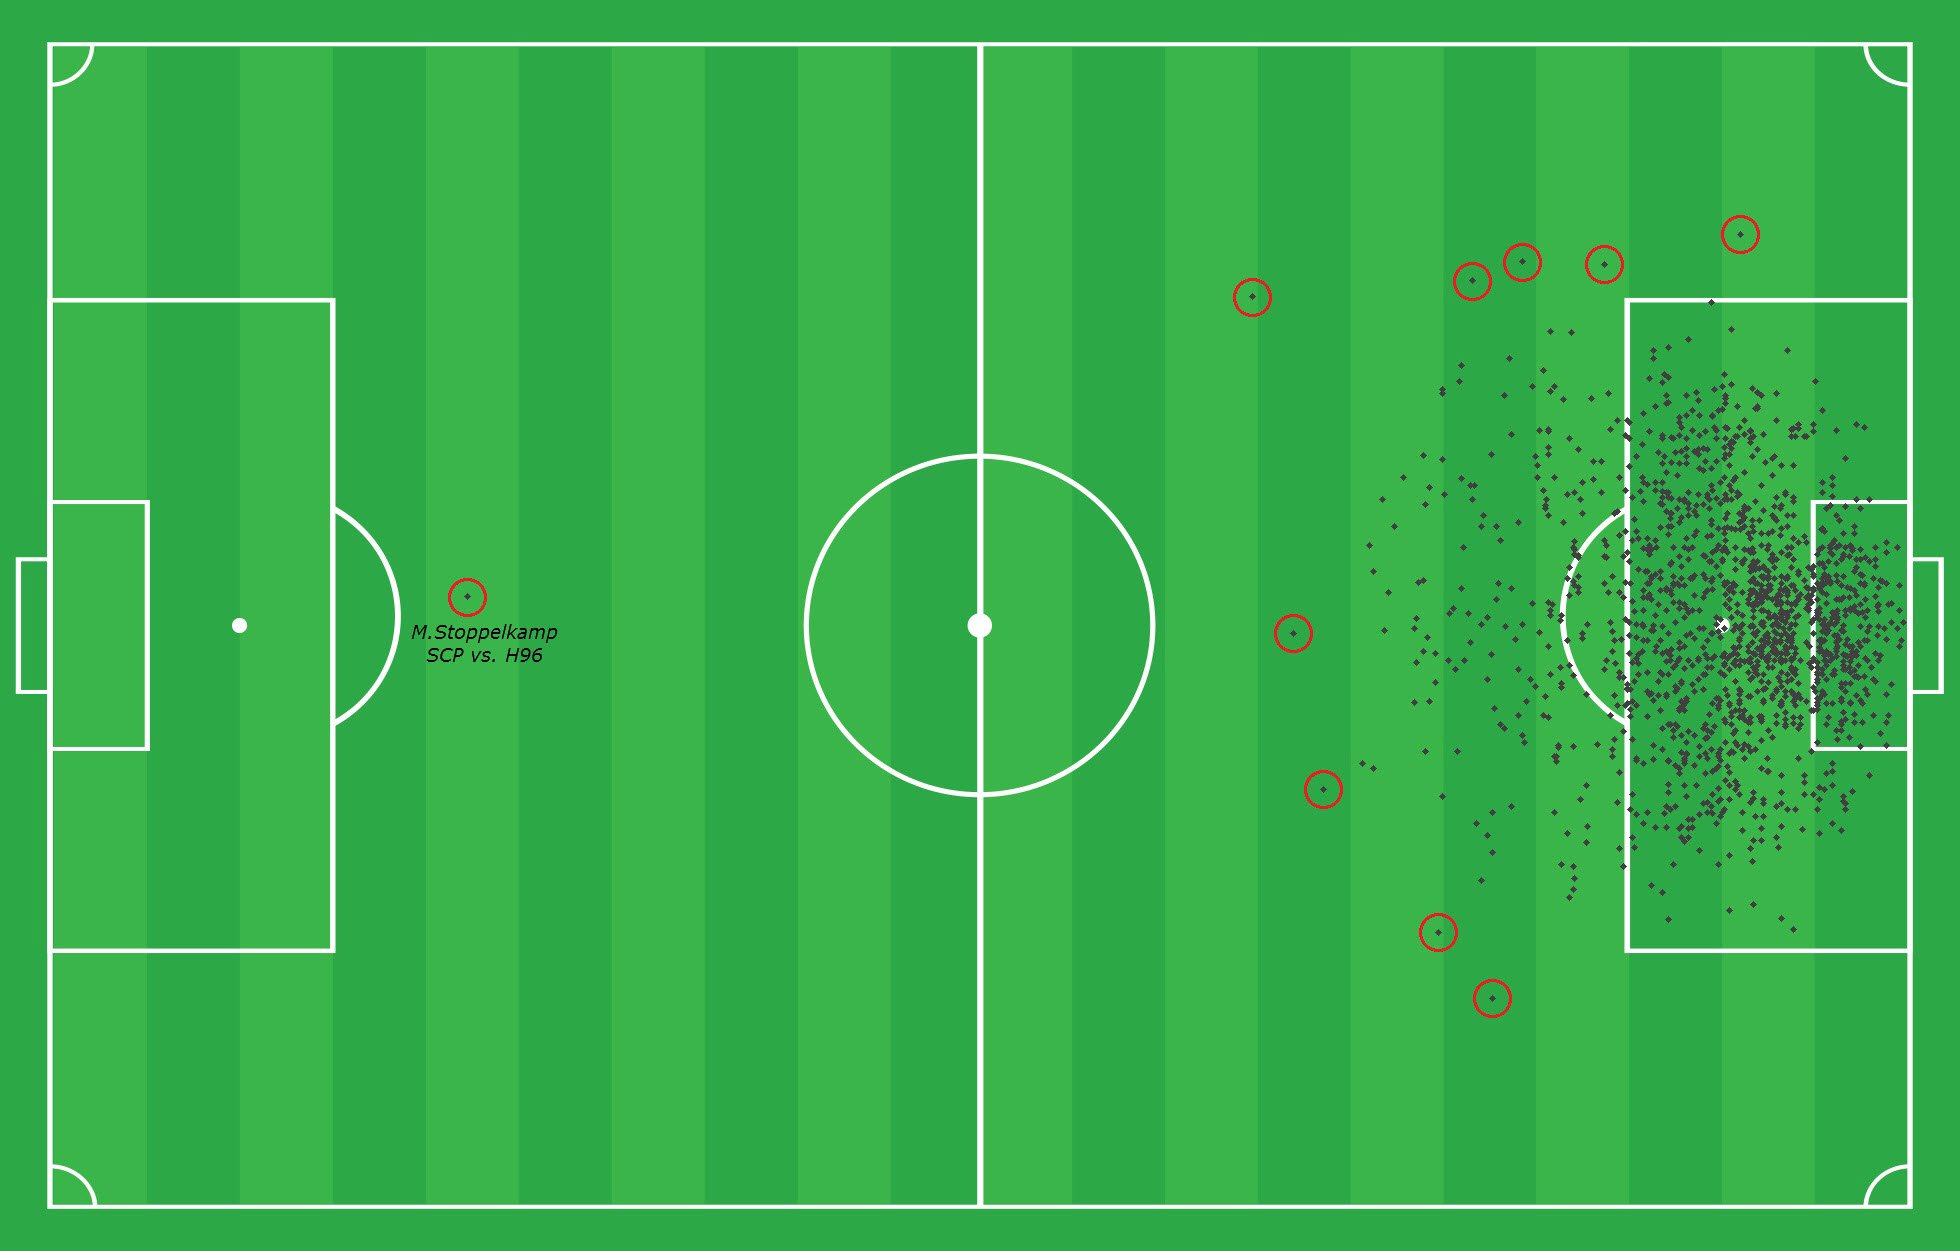
\includegraphics[scale=0.28]{se-wa-jpg/outlier_shots}
%\caption[Ausreißer bei Torerfolge]{Ausreißer bei Torerfolge}
%\label{outlier_shots}
%\end{figure}
